\documentclass[a4]{article}
% Nótese que el tanto por ciento sirve para comentar el resto de la lí­nea
%\usepackage[utf8]{inputenc}    % Válido en la mayorí­a de los casos
\usepackage[utf8]{inputenc}   % otra alternativa para los caracteres acentuados y la "ñ"
\usepackage[english
                      ,spanish % para poder usar el español
                      ,es-tabla % para los captions de las tablas
                       ]{babel}
\decimalpoint %para usar el punto decimal en vez de coma para los números con decimales

\usepackage{fancyvrb} % un interesante paquete para poder reproducir código LaTeX tal cual
\usepackage{fvextra}% otra opción que incluso completa el paquete anterior

\usepackage[T1]{fontenc}
\usepackage{lmodern}

\usepackage[official]{eurosym}  % para poder incluir el sí­mbolo del Euro

\usepackage{parskip}
\usepackage{xcolor}

\usepackage{enumerate}% paquete para poder personalizar fácilmente la apariencia de las listas enumerativas

\usepackage{graphicx} % figuras
\usepackage{subfigure} % subfiguras

\usepackage{rotating, graphicx}

\definecolor{gris}{RGB}{220,220,220}

\usepackage{pdfpages} % para poder introducir directamente páginas en PDF en el documento
	
\usepackage{float} % para controlar la situación de los entornos flotantes

\usepackage[pdftex,
bookmarks=true,
breaklinks,
pagebackref=true]{hyperref}

\usepackage{bookmark}

\restylefloat{figure}
\restylefloat{table}

\usepackage{blindtext}% para poder incluir cierto texto sin mucho sentido por defecto

\usepackage{rotating} % para rotar imágenes y otros elementos LaTeX
\usepackage{tikz} % uso del entorno tikzpicture

\newcommand{\HRule}{\rule{\linewidth}{1mm}}
\title
{
	\HRule
	\begin{flushright}
		\huge
		\textbf{Mi Tí­tulo}\\
		\Large
		\textbf{en}\\
		\Huge
		\textbf{Particular}\\
	\end{flushright}
	\HRule
}


\def\keywordsen{\vspace{.5em}
	{\textit{Keywords}:\,\relax%
}}
\def\endkeywordsen{\par}

\def\keywordses{\vspace{.5em}
	{\textit{Palabras clave}:\,\relax%
}}
\def\endkeywordses{\par}


\author{Pedro González Rodelas}
\date{}%{27/02/2018}
%\date{\vspace{-5ex}} % para eliminar el espacio que deja esta parte

\title{ Entornos estándard y algunos más especiales en \LaTeX}



\begin{document}

\maketitle
\thispagestyle{empty} % No pondrá cabecera, ni pie de página, ni numeración....

\selectlanguage{english}

\begin{abstract}
	\blindtext
\end{abstract}

\begin{keywordsen}
	 {\LaTeX} environments
\end{keywordsen}


\selectlanguage{spanish}

\begin{abstract}
	En este pequeño artí­culo, a modo de ensayo repasamos la mayor parte de los `entornos' fundamentales que se pueden encontrar y que configuran un fichero {\LaTeX} cualquiera. Aunque tomaremos como ejemplo tí­pico un documento de tipo {\tt article}, estos entornos fundamentales pueden aparecer en ficheros {\LaTeX} de cualquier tipo. Esto no impide que existan otros entornos más especí­ficos  que sólo tendrí­an sentido en otro tipo de documentos, como por ejemplo {\tt part} o {\tt chapter}, que se suelen usar más bien en los documentos de tipo  {\tt book} o {\tt report}.
\end{abstract}

\begin{keywordses}
	entornos {\LaTeX}
\end{keywordses}

\section{\contentsname}

\tableofcontents

\section{Introducción}

El entorno más fundamental que hay que considerar dentro de un documento {\LaTeX} es lo que se denomina el propio `cuerpo' del  mismo documento; es decir, todo lo que aparece encerrado entre

\verb+\begin{document}+

\vdots

\verb+\end{document}+

Otros entornos importantes muy empleados, sobre todo en el tipo de documento \verb+article+ son el Abstract (resumen que resalta lo más importante que se incluye en el artí­culo) y las Keywords (o palabras clave, por las que se podrá identificar dicho trabajo). Al igual que cualquier otro entorno de {\LaTeX} lo habitual es que se  comience con los correspondientes \verb+\begin{entorno}+ y  \verb+\end{entorno}+ con el nombre del entorno entre llaves.

También se podrí­a incluir o diseñar un entorno especial que defina una página inicial con el tí­tulo del trabajo, autor, fecha con los comandos correspondientes, pudiendo determinar a su vez la fuente y tamaño de la letra, cualquier imágen o logo, así­ como lí­neas decorativas o delimitadoras. He aquí­ un pequeño ejemplo

\begin{verbatim}
\begin{titlepage}
	\vspace*{4cm}
	{\fontsize{28}{34}\selectfont\bfseries Tí­tulo}
	\hfill
	% Logo
	\includegraphics[height=2cm]{example-image-b} \\
	% Lí­nea gris
	{\color{gris}\hrule}
	\Large{\itshape Subtí­tulo}
	\vfill
	{\large Autor \hfill Fecha}
\end{titlepage}
\end{verbatim}


cuyo resultado particularizado se puede ver ya en la página siguiente.

\begin{titlepage}
	\vspace*{4cm}
	{\fontsize{28}{34}\selectfont\bfseries \LaTeX}
	\hfill
	% Logo
	\includegraphics[height=2cm]{example-image-a} \\
	% Lí­nea gris
	{\color{gris}\hrule}
	\Large{\itshape Entornos básicos}
	\vfill
	{\large Autor: \hfill Fecha:}\\
	{\large Pedro González Rodelas \hfill \today}
\end{titlepage}

aunque otra opción muy usada podrí­a consistir en realizar dicha portada usando cierto software de maquetado especí­fico y generar un fichero en PDF, que después simplemente será importado con la correspondiente orden

\verb+\include{portada-PDF}+.

Otra posibilidad mucho más sofisticadaro para crear la portada, contraportada y lomo de un lib serí­a el uso del paquete \verb+bookcover+ (consultar por ejemplo

 \url{http://tug.ctan.org/macros/latex/contrib/bookcover/bookcover.pdf}).


 %\smallskip
 %\medskip
 %\bigskip
 %\vspace{4cm}
% \vskip 5 cm
 \vspace{2cm}


Probemos ahora la inclusión de caracteres acentuados, así­ como sí­mbolos y letras tí­picas del idioma español, como por ejemplo la letra `ñ'.

¡Hola mundo! ...............

\hspace{2cm}\vdots

Aquí­ estoy yo \ldots, en España.


%\end{document}

Vamos a seguir escribiendo en \LaTeX.

Otro de los entornos por antonomasia de {\LaTeX} es el entorno matemático, que será explicado en más profundidad más adelante, pero al que se puede acceder fácilmente entre sí­mbolos de dólar \$  \ldots \$, usando doble dólar para el modo resaltado y centrado.

Vea la diferencia entre escribir

Las soluciones de la ecuación de segundo grado
\verb|$ax^2+bx+c=0$|

son $x=\frac{-b\pm\sqrt{b^2-4ac}}{2a}$ (si escribimos \verb|$x=\frac{-b\pm\sqrt{b^2-4ac}}{2a}$|), o bien
$$x=\frac{-b\pm\sqrt{b^2-4ac}}{2a}$$
si escribimos \verb|$$x=\frac{-b\pm\sqrt{b^2-4ac}}{2a}$$|.

%\smallskip
%\medskip
\bigskip
%\vspace{4cm}
%\vskip 5 cm

Por otra parte, para ayudar a estructurar el documento conviene dividir éste en partes, capí­tulos, secciones, subsecciones, párrafos, etc.

Algunos ``entornos'' interesantes son también los siguientes:

{\tt itemize, enumerate, description, list, flushleft, flushright, center, quote, quotation, verse, verbatim, minipage, titlepage,  table, tabular, picture, figure, equation, eqnarray, array, thebibliography}

Otros ``entornos'' que también pueden ser usados dentro de otros son los siguientes:   {\tt  raggedleft, raggedright }

\section{El entorno {\tt itemize} }\label{sec:itemize}

Primero con las marcas que tenga por defecto.

\begin{itemize}\itemsep2pt
	\item Primer item
	\begin{itemize}\itemsep1pt
		\item Otro item más interno
		\begin{itemize}\itemsep1pt
		\item Otro item más interno aún
		\end{itemize}
	\end{itemize}	
	\item Segundo item
	\item Tercer item
\end{itemize}

vamos ahora a forzar una separación concreta entre los items con el comando

\verb+\begin{itemize}\itemsep4pt+

\begin{itemize}\itemsep5pt
	\item Primer item
	\item Segundo item
	\item Tercer item
\end{itemize}

y ahora con las marcas que queramos

\begin{itemize}
	\item[*] Primer item
	\item[-] Segundo item
	\item[.] Tercer item
\end{itemize}

aunque también es posible modificar los sí­mbolos por defecto que ya se tienen implementados, con los siguientes comandos

\begin{verbatim} % este es el entorno verbatim stándard de LaTeX explicado un poco más abajo
\renewcommand{\labelitemi}{$\bullet$}
\renewcommand{\labelitemii}{$\cdot$}
\renewcommand{\labelitemiii}{$\diamond$}
\renewcommand{\labelitemiv}{$\ast$}
\end{verbatim}

\renewcommand{\labelitemi}{$\bullet$}
\renewcommand{\labelitemii}{$\cdot$}
\renewcommand{\labelitemiii}{$\diamond$}
\renewcommand{\labelitemiv}{$\ast$}

\begin{itemize}
	\item Primer item
	\begin{itemize}
		\item Otro item más interno
		\begin{itemize}
			\item Otro item más interno aún
		\end{itemize}
	\end{itemize}	
	\item Segundo item
	\item Tercer item
\end{itemize}

\section{El entorno {\tt enumerate} }\label{sec:enumerate}

\begin{enumerate}
	\item Primer item
	\item Segundo item
	\item Tercer item
\end{enumerate}


para usar números romanos en mayúscula \verb+\begin{enumerate}[I]+

\begin{enumerate}[I]%
	\item Primer item
   \item Segundo item
   \item Tercer item
\end{enumerate}

para usar caracteres alfa-numéricos en minúsculas entre paréntesis comenzaremos con \verb+\begin{enumerate}[(a)]+

\begin{enumerate}[(a)]%
	\item Primer item
    \item Segundo item
   \item Tercer item
\end{enumerate}

para usar caracteres alfa-numéricos en mayúsculas entre paréntesis, comenzaremos con \verb+\begin{enumerate}[(A)]+

\begin{enumerate}[(A)]% .
	\item Primer item
    \item Segundo item
    \item Tercer item
\end{enumerate}


para usar números romanos en minúsculas entre paréntesis, empezaremos con
\verb+\begin{enumerate}[(i)]+

\begin{enumerate}[(i)]%
	\item Primer item
    \item Segundo item
    \item Tercer item
\end{enumerate}

\section{El entorno {\tt verbatim} }\label{sec:verbatim}

Si en algún momento queremos escribir algo que \LaTeX debe reproducir tal cual, entonces conviene incluirlo dentro de un entorno de tipo \verb|verbatim|, como por ejemplo

\verb+Esto se reproduce al pié de la letra (tipo máquina de escribir)+

\verb-Respetándose los espacios          que nosotros indiquemos.-

Respetándose los espacios          que nosotros indiquemos

Por ejemplo, ya podemos incluir en el fichero final caracteres especiales de \LaTeX, de manera que el compilador no los interprete sino que los muestre simplemente, como por ejemplo:
\verb|# $ % ^ _  ~ { } \|
Todos ellos se pueden obtener anteponiéndoles el carácter de barra invertida, o backlash (que se obtiene con el comando \verb|$\backslash$|), he aquí­ el efecto de dicho comando: $\backslash$.
Por ejemplo \$ , \_  \{, \}, \%, \#, \^~

\subsection{Usando el paquete {\tt fancyvrb}}\label{subsec:fancyvrb}

%\begin{Verbatim}%[curlyquotes]
%`quoted text'
%\end{Verbatim}

\begin{Verbatim}[curlyquotes]
`quoted text'
\end{Verbatim}

 \begin{Verbatim}[numbers=left, highlightlines={1, 3-4}]
   First line
   Second line
   Third line
   Fourth line
   Fifth line
   \end{Verbatim}

   \begin{Verbatim}[numbers=left, stepnumber=2,
                    numberfirstline]
   First line
   Second line
   Third line
   Fourth line
   \end{Verbatim}

%\smallskip
\medskip
%\bigskip
%\vspace{4cm}
%\vskip 5 cm

\begin{Verbatim}
1234567890
	1234567890123456789
		1234567890
	12345678901234567890
1234567890
\end{Verbatim}

\begin{Verbatim}[tabsize=4]
1234567890
	1234567890123456789
		1234567890
	12345678901234567890
1234567890
\end{Verbatim}


A partir de ahora podremos usar siempre que queramos este entorno {\tt verbatim} explicado en la Sección \ref{sec:verbatim}, ya sea en su forma habitual o bien mediante el paquete explicado en la subsección \ref{subsec:fancyvrb}.


\section{El entorno {\tt quote} }\label{sec:quote}

Vamos a continuación a ver algún ejemplo del entorno {\tt quote}

\begin{quote}
	El que escribe con {\LaTeX} debe prestar atención a no cometer errores...
\end{quote}

\begin{quotation}
	El que escribe con {\LaTeX} debe prestar atención a no cometer errores...
\end{quotation}

También está la opción de usar {\tt quotation} que sangra más los párrafos aunque los separa menos de lo habitual.


\section{El entorno {\tt description} }\label{sec:description}

\begin{description}
	
\item[Descripción] Vamos a describir algo aquí­ dentro
\item[Otra descripción] Aquí­ tenemos una descripción equivalente
	
\end{description}

\section{El entorno {\tt  flushleft} }\label{sec:flushleft}

Sirve para alinear tanto texto como fórmulas matemáticas a la izquierda.

\begin{flushleft}
	\textbf{Trozo de texto alineado a la izquierda:} \\
   \blindtext
\end{flushleft}


\begin{flushleft}
	\textbf{Ejemplos de términos alineados a la izquierda:} \\
	$3x$ y $5x$ \\
	$4y^2$ y $9y^2$ \\
	$7xy$ y $3xy$ \\
	$6$ y $15$
\end{flushleft}

\section{El entorno {\tt flushright} }\label{sec:flushright}

Sirve para alinear tanto texto como fórmulas matemáticas a la derecha.

\begin{flushright}
	\textbf{Trozo de texto alineado a la derecha:} \\
	\blindtext
\end{flushright}

\begin{flushright}
	\textbf{Ejemplos de términos alineados a la derecha:} \\
	$2x$ y $8y$ \\
	$4t^2$ y $4t^3$ \\
	$x^2y$ y $xy^2$ \\
	$12$ y $12x$
\end{flushright}

\section{El entorno {\tt center} }\label{sec:center}

Sirve para centrar tanto texto como fórmulas matemáticas.

\begin{center}
	\textbf{Trozo de texto centrado:} \\
	\blindtext
\end{center}

\begin{center}
	\textbf{Ejemplos de términos centrados:} \\
	$2x$ y $8y$ \\
	$4t^2$ y $4t^3$ \\
	$x^2y$ y $xy^2$ \\
	$12$ y $12x$
\end{center}


\section{El entorno {\tt minipage} }\label{sec:minipage}

\begin{minipage}{.45\linewidth}
\begin{flushleft}
	\textbf{Ejemplos de términos alineados a la izquierda:} \\
	$3x$ y $5x$ \\
	$4y^2$ y $9y^2$ \\
	$7xy$ y $3xy$ \\
	$6$ y $15$
\end{flushleft}
\end{minipage}
\hfill
\begin{minipage}{.45\linewidth}
\begin{flushright}
	\textbf{Ejemplos de términos alineados a la derecha:} \\
	$2x$ y $8y$ \\
	$4t^2$ y $4t^3$ \\
	$x^2y$ y $xy^2$ \\
	$12$ y $12x$
\end{flushright}
\end{minipage}

\section{El entorno {\tt tabbing} }\label{sec:tabbing}

{\bf El entorno tabbing} produce texto alineado en columnas de forma similar a los tabuladores de una máquina de escribir\footnote{Conviene aclarar que \ldots}



\begin{tabbing}
Nombre   \= Apellido    \=   Teléfono \\
Juan   \>  Gómez \> 3141592 \\
Pedro  \>  Sáenz \> 2718281
\end{tabbing}

\begin{tabbing}
	Nombrexxxxxxxxxx   \= Apellidoxxxxxxx    \=   Teléfonoxxxxxxxx  \kill
	Nombre   \> Apellido    \>   Teléfono \\
	Juan   \>  Gómez \> 3141592 \\
	Pedro  \>  Sáenz \> 2718281
\end{tabbing}


Veámos cómo añadir cierto margen a la izquierda con el comando %\verb{  \+ }

\begin{tabbing}
margen xxxxx\=	Nombrexxxxxxxxxx   \= Apellidoxxxxxxx    \=   Teléfonoxxxxxxxx\+ \kill
	Nombre   \> Apellido    \>   Teléfono \\
	Juan   \>  Gómez \> 3141592 \\
	Pedro  \>  Sáenz \> 2718281
\end{tabbing}

\section{El entorno {\tt verse} }\label{sec:verse}

\begin{verse}
En la orilla del rí­o \\
hay un sapo\\
voy a cogerlo\\
y se me escapa.
\end{verse}

\section{El entorno {\tt tabular} }\label{sec:tabular}

Veámos algunos ejemplos básicos del entorno {\tt tabular} que intentaremos reproducir poco a poco, o al principio con la ayuda de alguna herramienta online, como las que siguen:

 \url{http://truben.no/table/old/}).

  \url{https://www.tablesgenerator.com}).

  \vspace{0.5cm}

\begin{center}
  \begin{tabular}{l*{6}{c}r}
	Team              & P & W & D & L & F  & A & \euro \\\hline
	Manchester United & 6 & 4 & 0 & 2 & 10 & 5 & 12  \\
	Celtic            & 6 & 3 & 0 & 3 &  8 & 9 &  9  \\
	Benfica           & 6 & 2 & 1 & 3 &  7 & 8 &  7  \\
	FC Copenhagen     & 6 & 2 & 1 & 3 &  5 & 8 &  7  \\
\end{tabular}
\end{center}
\vspace{0.5cm}

\begin{center}
	\begin{tabular}{|r|l|}
		\hline
		7C0         & hexadecimal \\
		3700        & octal       \\ \cline{2-2}
		11111000000 & binary      \\
		\hline\hline
		1984        & decimal     \\
		\hline
	\end{tabular}
\end{center}
\vspace{0.5cm}

\begin{center}
	\begin{tabular}{|p{4.7cm}|}
		\hline
		Welcome to Boxy?s paragraph.
		We sincerely hope you?ll
		all enjoy the show.\\
		\hline
	\end{tabular}
\end{center}
\vspace{0.5cm}

\begin{center}
\begin{minipage}{.45\linewidth}
	\begin{flushleft}
		\textbf{Tabla generada con {\tt tablesgenerator.com}:} \\

	\begin{tabular}{|l|l|l|}
	\hline
	& \multicolumn{2}{l|}{columnas} \\ \hline
	1  & 2             & 3             \\ \cline{2-3}
	14 & 15            & 16            \\ \hline
	7  & 8             & 9             \\ \hline
\end{tabular}
	\end{flushleft}
\end{minipage}
\hfill
\begin{minipage}{.45\linewidth}
	\begin{flushright}
		\textbf{Tabla generada a mano:} \\

  \begin{tabular}{|l|c||r|}
	\hline
	&\multicolumn{2}{c|}{\tiny columnas}\\\hline
	1 &  2 & 3  \\\cline{2-3}
	14 & 15 & 16 \\\hline\hline
	7 &  8 & 9  \\
	\hline
\end{tabular}

	\end{flushright}
\end{minipage}
\end{center}
\vspace{1cm}

\begin{center}
	
	\textbf{Ejemplos de términos alineados usando {\tt tabular}}
	
	\begin{tabular*}{\textwidth}{@{}l@{\extracolsep{\fill}}r@{}}
		\textbf{a la izquierda:}  & \textbf{ a la derecha:} \\
		$3x$ y $5x$           &   $2x$ y $8y$ \\
		$4y^2$ y $9y^2$   &   $4t^2$ y $4t^3$ \\
		$7xy$ y $3xy$       &   $x^2y$ y $xy^2$ \\
		$6$ y $15$             &   $12$ y $12x$
	\end{tabular*}
\end{center}

\section{El entorno {\tt table} }\label{sec:table}

\begin{table}[hptb]
	\centering
	\caption{Errores e í­ndices de similaridad.}
	\label{TablaErrores}
	{\begin{tabular}[h]{|l |c |c |c |c| }
			\hline
			Valores de $n=m$ & $\overline S_d$ & $\overline{S}_{CHEN}$ & $\overline{S}_{HSIEH}$ & $\overline{S}_{SCGM}$ \\
			\hline
			\centering
			$4$ & $7.8692\times 10^{-2}$ & $0.949328$ & $0.955893$ & $0.955190$\\
			\hline
			$6$ & $2.7178\times 10^{-2}$ & $0.981314$ & $0.982188$ & $0.982048$\\
			\hline
			$8$ & $9.8117\times 10^{-3}$ & $0.992527$ & $0.993364$ & $0.993119$\\
			\hline
			$10$ & $5.4005\times 10^{-3}$ & $0.995724$ & $0.996427$ & $0.996109$\\
			\hline
			$12$ & $3.0842\times 10^{-3}$ & $0.997768$ & $0.997906$ & $0.997895$\\
			\hline
			$20$ & $6.9539\times 10^{-4}$ & $0.999533$ & $0.999617$ & $0.999539$\\
			\hline
	\end{tabular}}
\end{table}


Otras opciones más avanzadas de crear tablas especiales son mediante los paquetes {\tt tabularx}, {\tt tabulary} y {\tt booktabs}. Consultar los manuales correspondientes o la abundante información disponible online.

\section{El entorno {\tt figure} }\label{sec:figure}

\begin{figure}[H]%[!hbtp]
	\centering
	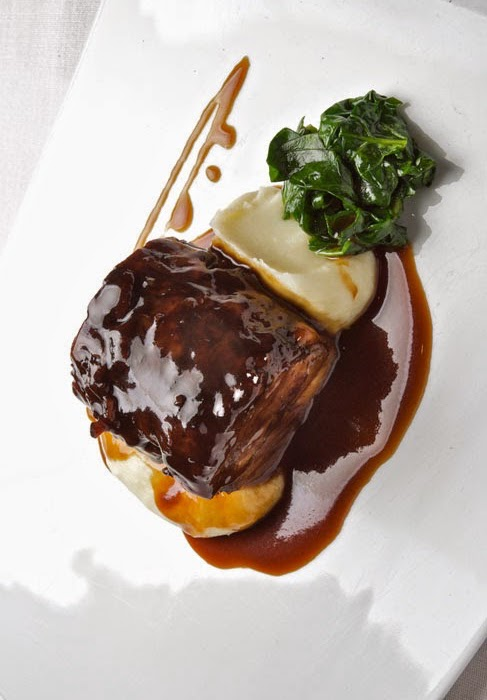
\includegraphics[width=4cm]{figs/rabo_toro_estofado}
	\caption{\scriptsize{Ejemplo de figura}}
	\label{fig:rabo_toro}
\end{figure}

\begin{figure}[H]
	\centering
\begin{turn}{-90}
	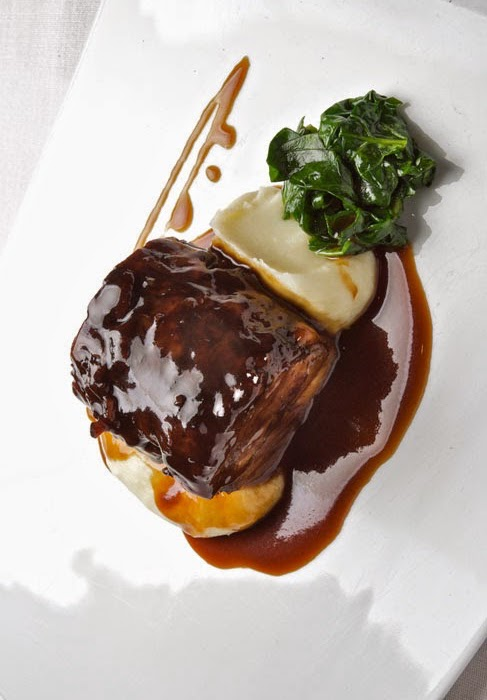
\includegraphics[width=8cm]{figs/rabo_toro_estofado}
\end{turn}
	\caption{\scriptsize{Ejemplo de figura rotada}}
\label{fig:rabo_toro_rotada}
\end{figure}

\section{Rotando otros objetos \LaTeX}\label{sec:rot_objetos}

Aunque también podrí­amos haber rotado cualquier otro objeto de {\LaTeX} como por ejemplo un trozo de texto insertado en una minipágina, o una tabla cualquiera, como la de la sección anterior \ref{sec:table}.

\begin{turn}{45}
	\begin{minipage}{\linewidth}
		\blindtext
	\end{minipage}
\end{turn}
\bigskip
\newline
\blindtext


\begin{minipage}{.45\linewidth}
	\begin{flushleft}
		\textbf{Ejemplos de términos alineados a la izquierda:} \\
		$3x$ y $5x$ \\
		$4y^2$ y $9y^2$ \\
		$7xy$ y $3xy$ \\
		$6$ y $15$
	\end{flushleft}
\end{minipage}
\hfill
\begin{minipage}{.45\linewidth}
	\begin{flushright}
		\textbf{Ejemplos de términos alineados a la derecha:} \\
		$2x$ y $8y$ \\
		$4t^2$ y $4t^3$ \\
		$x^2y$ y $xy^2$ \\
		$12$ y $12x$
	\end{flushright}
\end{minipage}



\begin{table}[hptb]
	\centering
	\begin{turn}{45}
	\caption{Errores e í­ndices de similaridad.}
	\label{TablaErrores_rotada}
	{\begin{tabular}[h]{|l |c |c |c |c| }
			\hline
			Valores de $n=m$ & $\overline S_d$ & $\overline{S}_{CHEN}$ & $\overline{S}_{HSIEH}$ & $\overline{S}_{SCGM}$ \\
			\hline
			\centering
			$4$ & $7.8692\times 10^{-2}$ & $0.949328$ & $0.955893$ & $0.955190$\\
			\hline
			$6$ & $2.7178\times 10^{-2}$ & $0.981314$ & $0.982188$ & $0.982048$\\
			\hline
			$8$ & $9.8117\times 10^{-3}$ & $0.992527$ & $0.993364$ & $0.993119$\\
			\hline
			$10$ & $5.4005\times 10^{-3}$ & $0.995724$ & $0.996427$ & $0.996109$\\
			\hline
			$12$ & $3.0842\times 10^{-3}$ & $0.997768$ & $0.997906$ & $0.997895$\\
			\hline
			$20$ & $6.9539\times 10^{-4}$ & $0.999533$ & $0.999617$ & $0.999539$\\
			\hline
	\end{tabular}}
\end{turn}
\end{table}


También podemos usar el package \verb+float+ con la opción \verb+[H]+

%\end{document}

\begin{figure}[H]
	\centering
	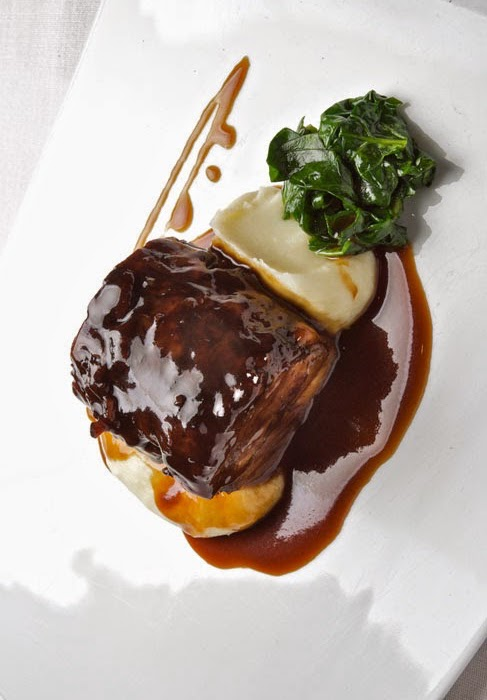
\includegraphics[width=12cm]{figs/rabo_toro_estofado}
	\caption{Aquí­ se escribe el pié de página}\label{fig:rabotoro3}
\end{figure}

Otras opciones serí­an el uso del entorno minipage y el paquete caption

\begin{Verbatim}
\usepackage{caption}
...
\noindent%
\begin{minipage}{\linewidth}
% para mantener tanto la imagen como el pié (caption) en una página
\makebox[\linewidth]{%     para centrar la imagen
\includegraphics[keepaspectratio=true,scale=0.6]%{figura}}
\captionof{figure}{...}\label{fig:rabotoro4}%  sólo si se necesita
\end{minipage}
\end{Verbatim}

o bien

\begin{Verbatim}
\begin{center}
\includegraphics[...]{figura}}
\captionof{figure}{...}\label{fig:}% sólo si se necesita
\end{center}
\end{Verbatim}

\subsection{Incluyendo una página completa usando {\tt pdfpages} }\label{subsec:pdfpages}

En este caso habrí­a que haber cargado previamente el paquete correspondiente, mediante el comando

\verb|\usepackage{pdfpages}|

y en el lugar apropiado del fichero fuente incluir ahora

\verb|\includepdf[pages={1}]{fichero.pdf}]|.

La página o páginas incluidas aparecerán a partir de la página siguiente, como puede comprobar.

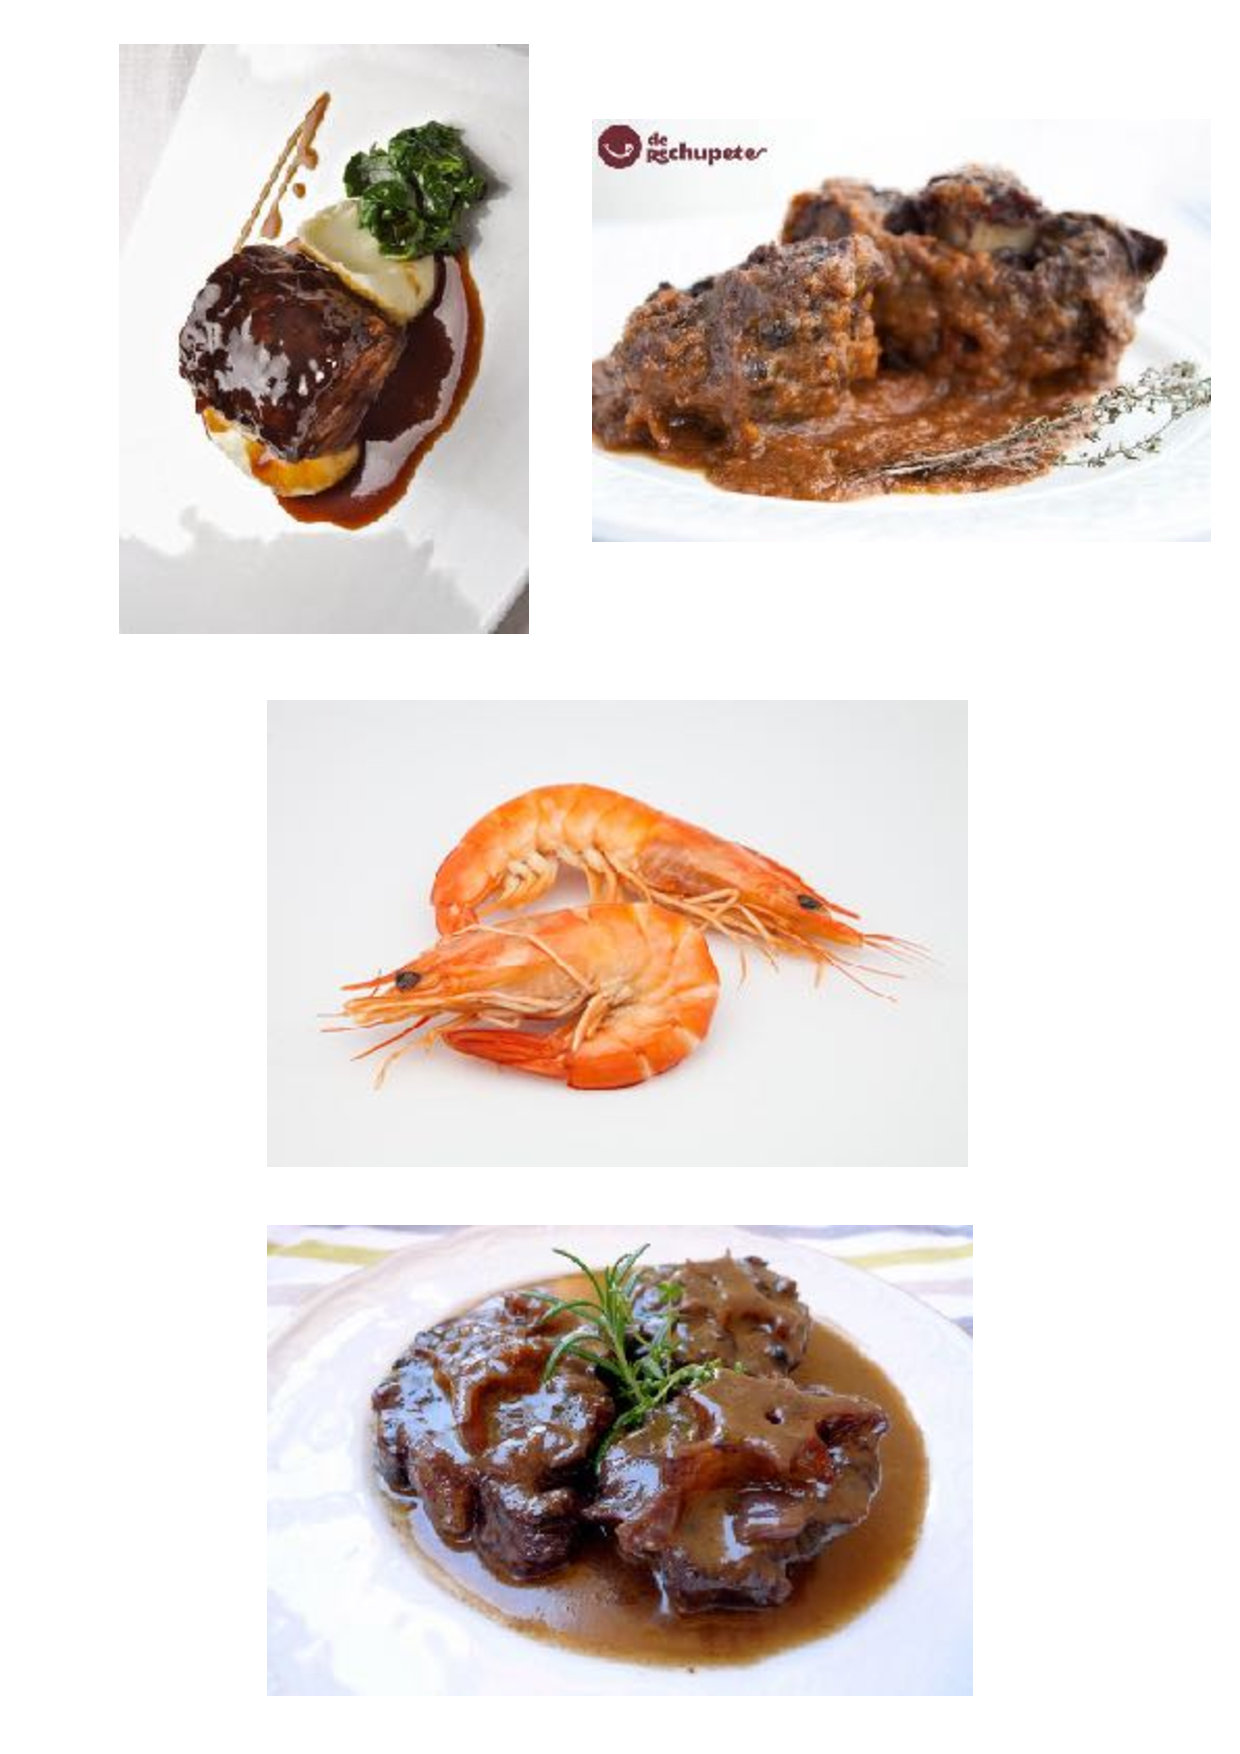
\includepdf[pages={1}]{figs/RaboToroyLangostinos}]

\subsection{El entorno {\tt subfigure} }\label{subsec:subfigure}

Este entorno permite añadir una especie de lista de figuras, cada una con un pequeño pié de figura, aparte irí­a un {\tt caption} común, ya sea abajo o arriba del grupo de subfiguras.  Si quieres que vaya arriba, basta con que escribas la etiqueta \verb+\caption{}+ antes de \verb+\includegraphics[]{}+.
%\end{document} %%%%%%%%%%%%%%%%%%%%%%%%%%%%%%%%%%%%%%%%%%%%%%%%%%

\begin{figure}[htbp]
	\centering
	\subfigure[Langostinos 1]{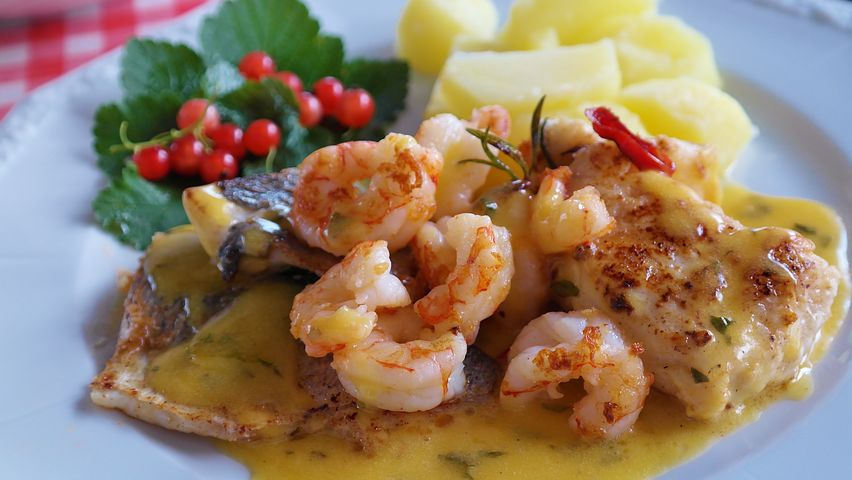
\includegraphics[width=40mm]{figs/langostinos1}}
	\subfigure[Langostinos 2]{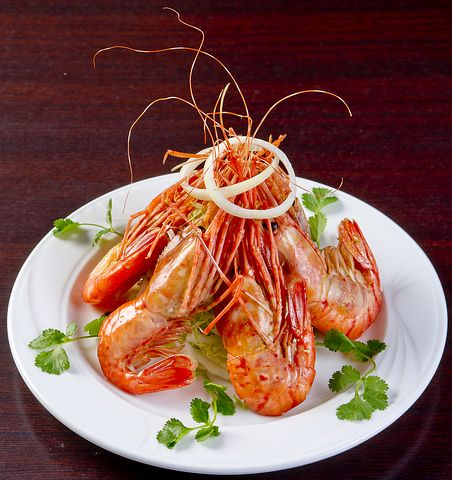
\includegraphics[width=40mm]{figs/langostinos2}}
	\subfigure[Langostinos 3]{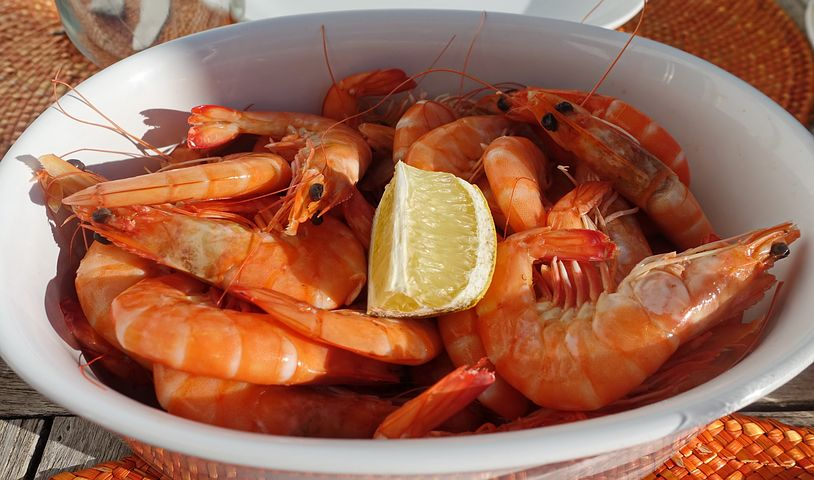
\includegraphics[width=80mm]{figs/langostinos3}}
	\caption{Langostinos.} \label{fig:langostinos}
\end{figure}


\begin{figure}[htbp]	 \label{fig:langostinos}

	\caption{Distintas formas de preparar los langostinos.}
	\centering
	\subfigure[Langostinos 1]{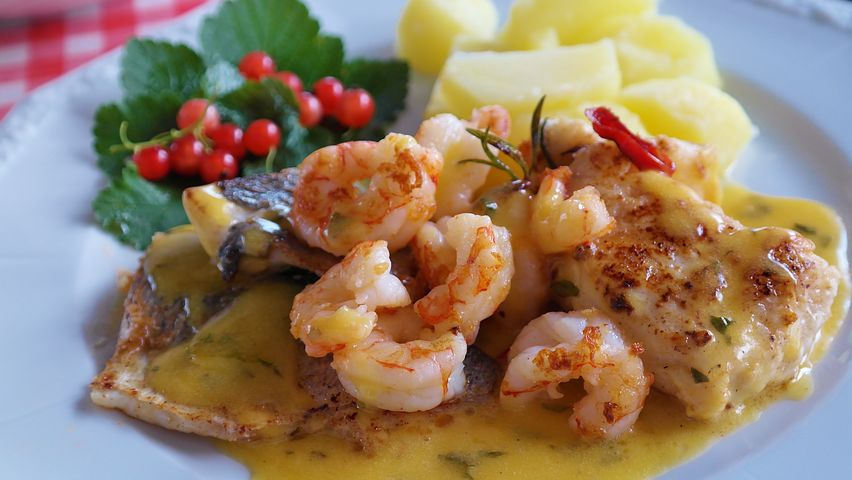
\includegraphics[width=40mm]{figs/langostinos1}}
	\subfigure[Langostinos 3]{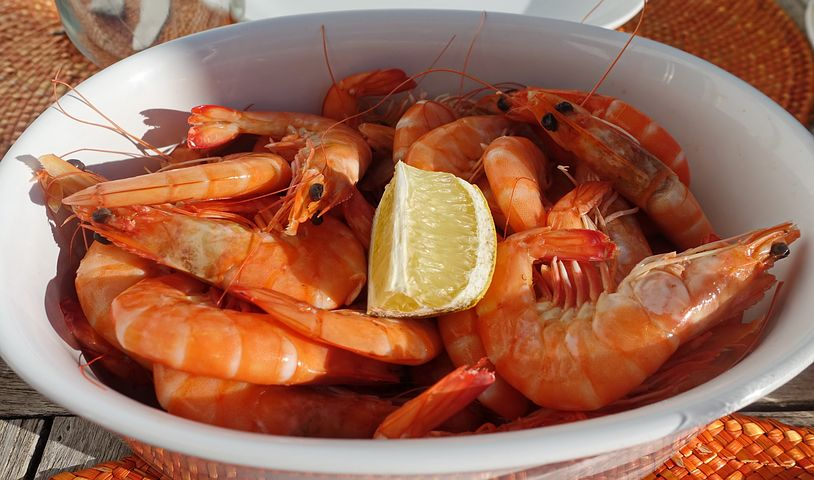
\includegraphics[width=40mm]{figs/langostinos3}}\\
	\subfigure[Langostinos 2]{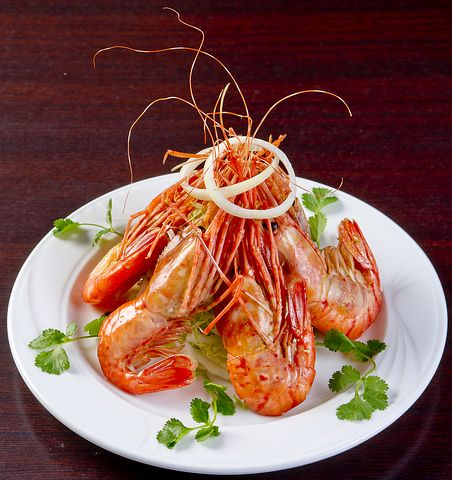
\includegraphics[width=80mm]{figs/langostinos2}}
\end{figure}

Para separar las subfiguras entre sí­, puedes usar \verb+\vspace+ y \verb+\hspace+, para modificar el espacio vertical y horizontal respectivamente:


\begin{figure}[htbp]
	\centering
	\subfigure[Langostinos 1]{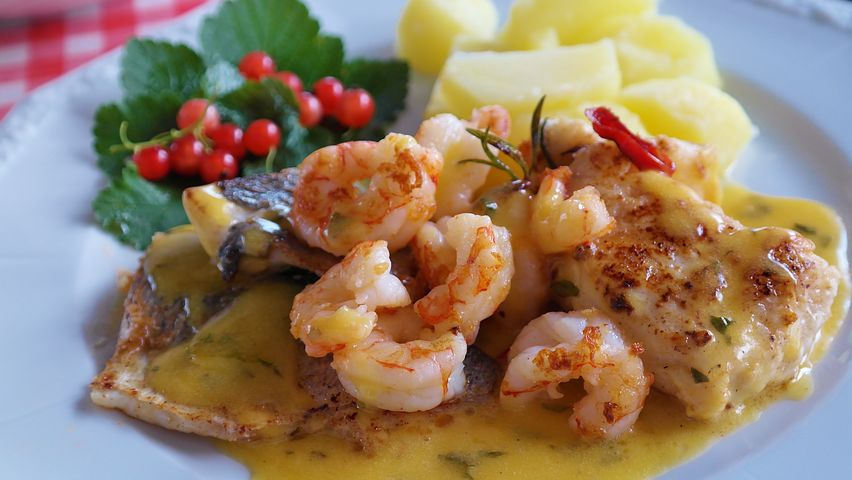
\includegraphics[width=40mm]{figs/langostinos1}}\hspace{10mm}
	\subfigure[Langostinos 2]{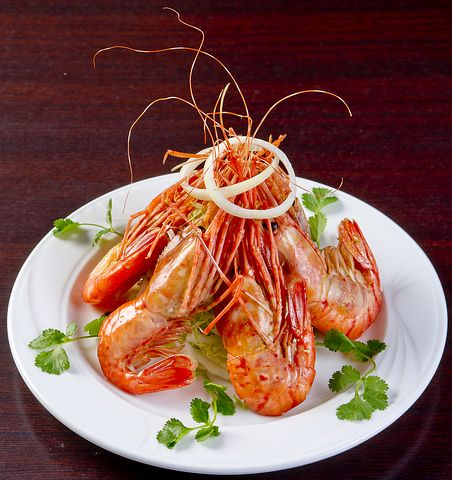
\includegraphics[width=40mm]{figs/langostinos2}}\vspace{10mm}
	\subfigure[Langostinos 3]{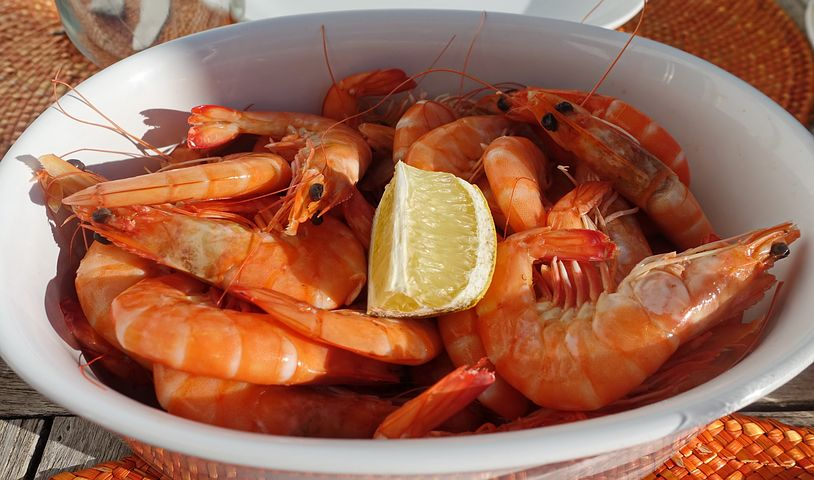
\includegraphics[width=80mm]{figs/langostinos3}}
	\caption{Langostinos más separados} \label{fig:langostinossep}
\end{figure}

\vspace*{2cm}

\subsection{Para organizar las figuras en una tabla o {\tt grid} }\label{subsec:gridfigures}

\begin{table}[H]
	\centering
\begin{tabular}{cc}
 {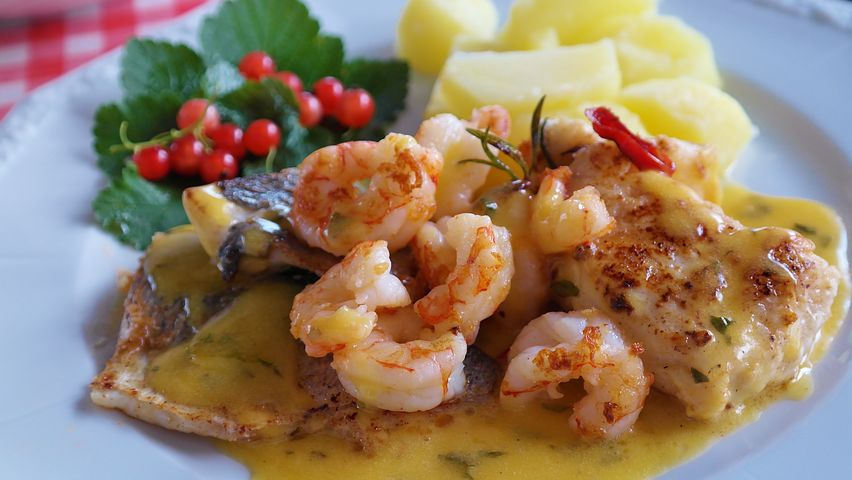
\includegraphics[width=40mm]{figs/langostinos1}} & {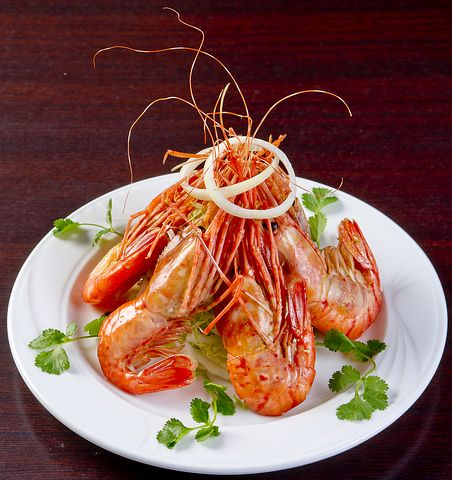
\includegraphics[width=40mm]{figs/langostinos2}} \\
                                 & {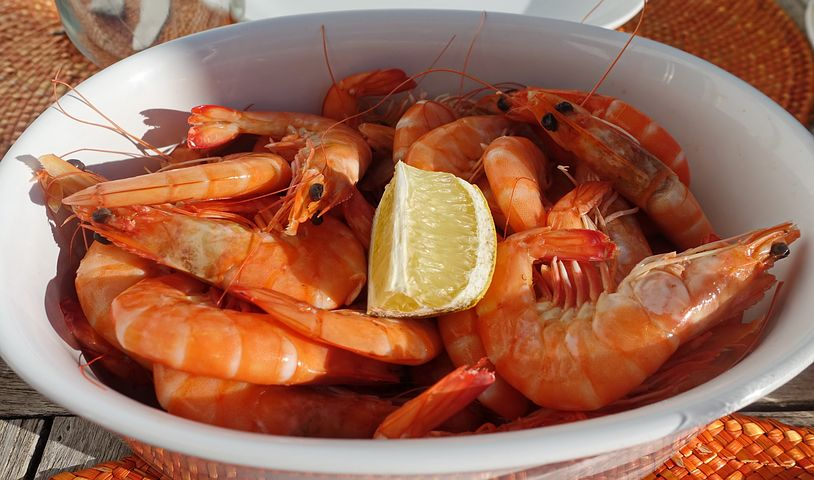
\includegraphics[width=40mm]{figs/langostinos3}}
\end{tabular}
\caption{Organizando figuras a modo de tabla.}
\end{table}


\begin{table}[H]
	\centering
	\begin{tabular}{cc}
		\subfigure[Langostinos 1]{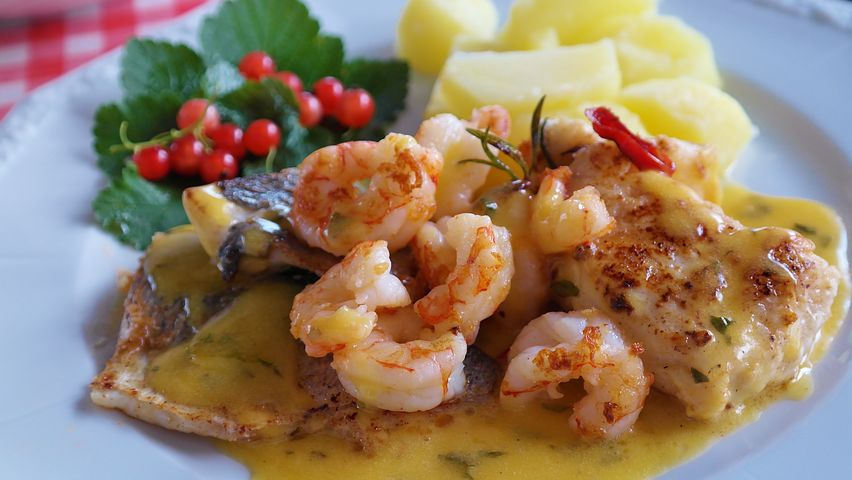
\includegraphics[width=40mm]{figs/langostinos1}} & \subfigure[Langostinos 2]{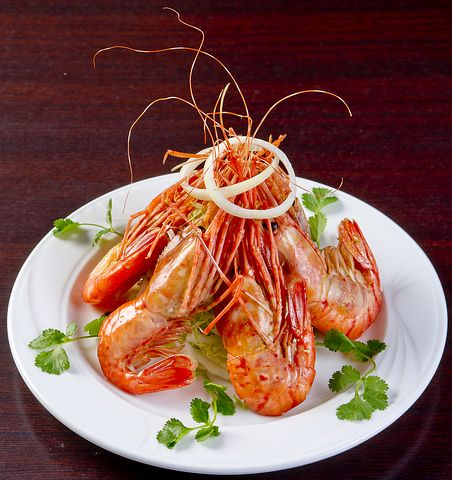
\includegraphics[width=40mm]{figs/langostinos2}} \\
		& \subfigure[Langostinos 3]{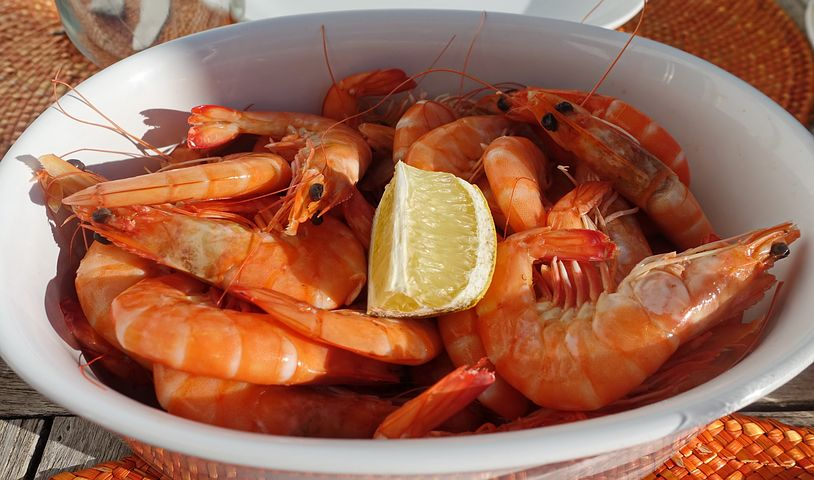
\includegraphics[width=40mm]{figs/langostinos3}}
	\end{tabular}
	\caption{Organizando figuras a modo de tabla.}
\end{table}

\section{El entorno {\tt picture} }\label{sec:picture}

\subsection{El entorno {\tt tikzpicture} }\label{subsec:tikzpicture}

\begin{figure}[H]%[!htbp]
	\centering
	\begin{tikzpicture}[scale=4]
	\fill[blue] (0,0) rectangle(2,1.5);
	\end{tikzpicture}	
	\caption{Figura generada con el paquete {\tt tikz}}
	\label{fig:tikz_picture}
\end{figure}

\section*{Bibliografí­a}

Ya por último incluimos alguna bibliografí­a a modo de ejemplo.

\begin{thebibliography}{10}
	
	
	
	
	\bibitem{Lamport} L. Lamport, {\LaTeX}: A Document Preparation System (2nd Ed.).
	
	\bibitem{Goossens} M. Goossens, F. Mittelbach, A. Samarin, The  {\LaTeX} Companion. Addison-Wesley Publishing Company (2002).
	
	\bibitem{} M. Goossens, F. Mittelbach, S. Rahtz, D. Roegel, H. Vo$\beta$, The  {\LaTeX} Graphics Companion (2nd Ed.). Addison-Wesley Publishing Company (2007).
	
\end{thebibliography}

\end{document}

